 \documentclass{article}
\usepackage{pgf-umlcd}
\begin{document}
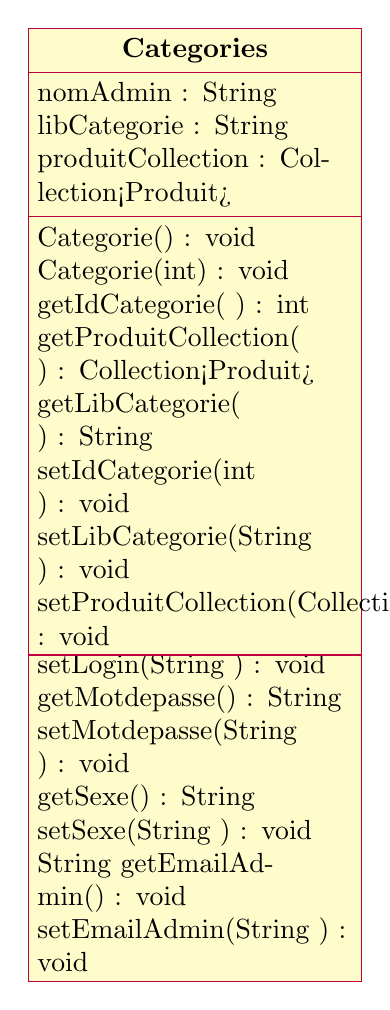
\begin{tikzpicture} 
%administrateur%
\begin{class}[text width=4cm,]{Administrateur}{0,0} 
\attribute{nomAdmin : String} 
\attribute{prenomAdmin : String} 
\attribute{login : String} 
\attribute{motdepasse : String} 
\attribute{sexe : String} 
\attribute{emailAdmin : String} 
\operation{Administrateur() : void} 
\operation{Administrateur(String) : void} 
\operation{getNomAdmin() : void} 
\operation{setNomAdmin(String ) : void} 
\operation{getPrenomAdmin() : String} 
\operation{setPrenomAdmin(String ) : void} 
\operation{getLogin() : String} 
\operation{setLogin(String ) : void} 
\operation{getMotdepasse() : String} 
\operation{setMotdepasse(String ) : void} 
\operation{getSexe() : String} 
\operation{setSexe(String ) : void} 
\operation{String getEmailAdmin() : void} 
\operation{setEmailAdmin(String ) : void} 

\end{class} 
\begin{class}[text width=4cm,]{Categories}{0,0} 
\attribute{nomAdmin : String} 
\attribute{libCategorie : String} 
\attribute{produitCollection : Collection<Produit>} 
\operation{Categorie() : void} 
\operation{Categorie(int) : void}
\operation{getIdCategorie( ) : int} 
\operation{getProduitCollection( ) : Collection<Produit>} 
\operation{getLibCategorie( ) : String} 
\operation{setIdCategorie(int ) : void} 
\operation{setLibCategorie(String ) : void}
\operation{setProduitCollection(Collection<Produit>) : void} 
\end{class} 
\end{tikzpicture}
\end{document}